\documentclass{article}
\usepackage{amsmath}
\usepackage{amsfonts}
\usepackage{bm}
\usepackage{graphicx}
\usepackage{float}
\usepackage{subfigure}
\usepackage{enumitem}
\usepackage{ctex}

\title{Wireless Communication Systems  HW2\\109064509 楊暐之}
\date{}
\renewcommand{\figurename}{Figure}
\renewcommand{\thesubfigure}{}

\begin{document}
\maketitle
\begin{flushleft}
We have the Doppler frequency shift formula
\begin{equation}
f_{D,n}(t)=f_m\cos\theta_n(t) \notag
\end{equation}
where $f_m=\frac{v}{\lambda_c}$ and $\lambda_c$ is the wavelength\\
Furthermore, $\lambda_c=\frac{c}{f_c}\Rightarrow f_m=\frac{vf_c}{c}$ where $c$ is the speed of light\\[0.2cm]
For the subproblems (a) and (b) of problem 1, I sample $F_{D,n}(t)=f_m\cos\Theta$ 100000 times and divide $[-fm,fm]$ into 10000 subintervals and then count how many samples lie in each subinterval so that simulate the pdf of $F_{D,n}(t)$\\
(Instead of $[-fm,fm]$, I use the minimum and maximum of sample to build the interval)\\[0.2cm]
For the subproblem (c), I assume $V$ and $\Theta$ are independent so it just need sampling $V$ and $\Theta$ respectively and componentwise multipling the samples of $V$ by those of $\Theta$ to get new samples. Then, do the same thing as (a) and (b)

\newpage

\begin{enumerate}[label=(\alph*)]
\item
 $v$=20km/h, $f_c$=2GHz
\begin{figure}[H]
\centering
\subfigure[pdf]{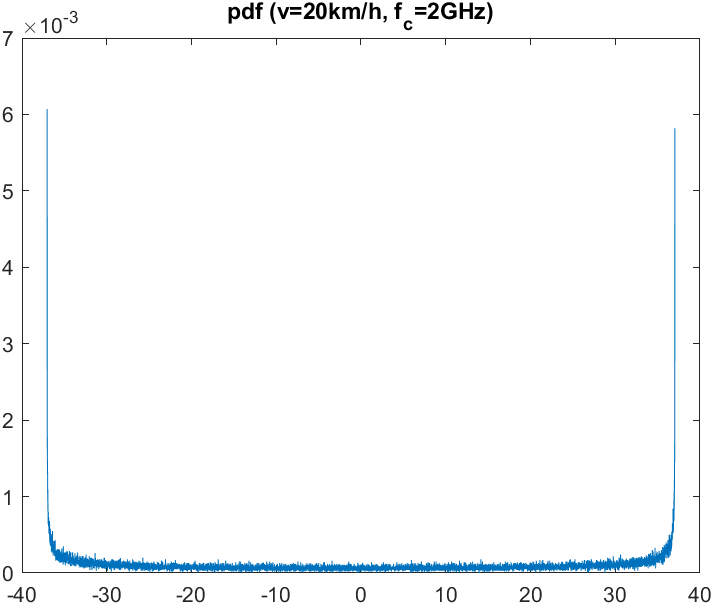
\includegraphics[width=0.49\textwidth]{(a)_pdf}}
\subfigure[cdf]{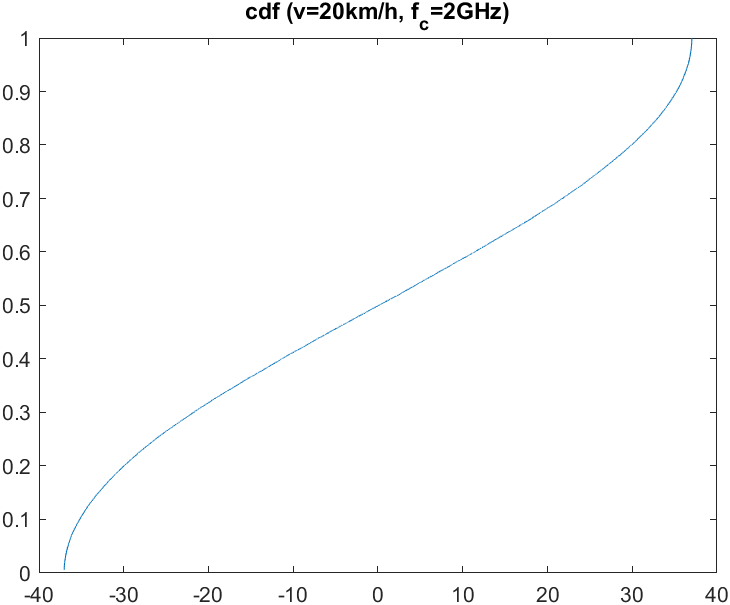
\includegraphics[width=0.49\textwidth]{(a)_cdf}}
\caption{ $v$=20km/h, $f_c$=2GHz}
\end{figure}

\item 
$v$=90km/h, $f_c$=26GHz
\begin{figure}[H]
\centering
\subfigure[pdf]{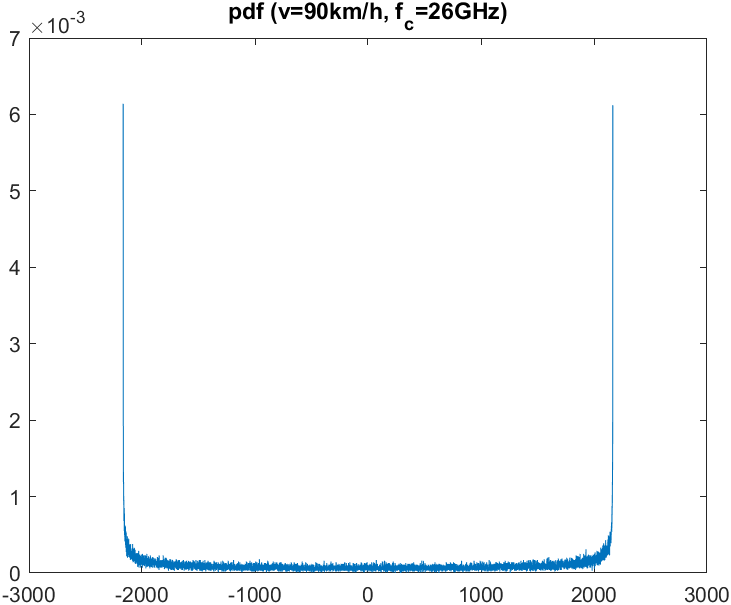
\includegraphics[width=0.49\textwidth]{(b)_pdf}}
\subfigure[cdf]{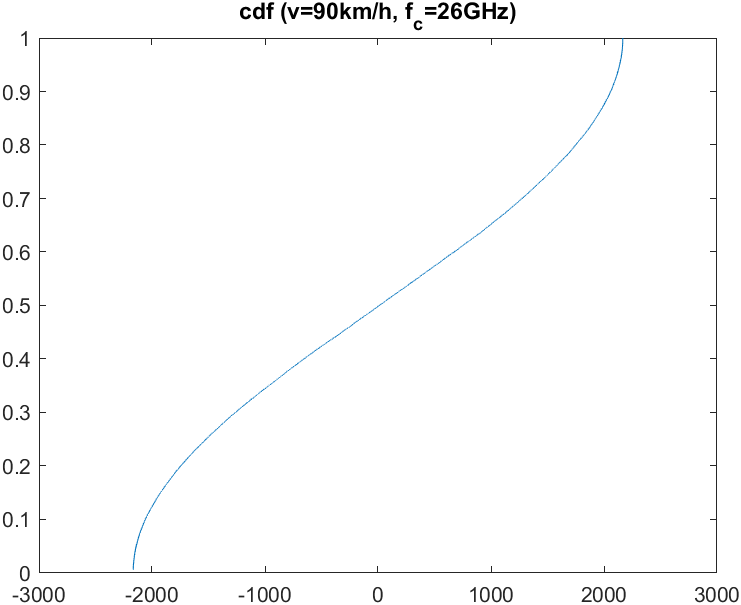
\includegraphics[width=0.49\textwidth]{(b)_cdf}}
\caption{ $v$=90km/h, $f_c$=26GHz}
\end{figure}

\newpage

\item 
$V\sim U(20,90)$km/h, $f_c$=2GHz\\
Here, I ssume $V$ and $\Theta$ are independent
\begin{figure}[H]
\centering
\subfigure[pdf]{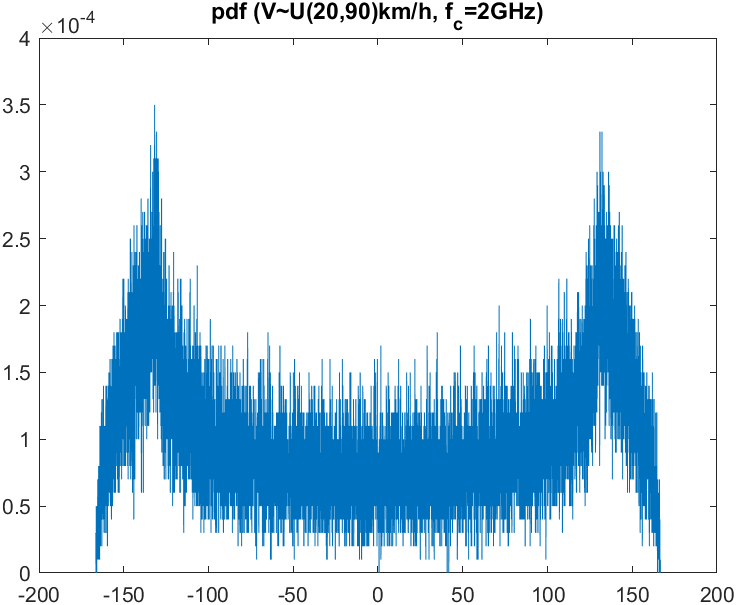
\includegraphics[width=0.49\textwidth]{(c)_pdf}}
\subfigure[cdf]{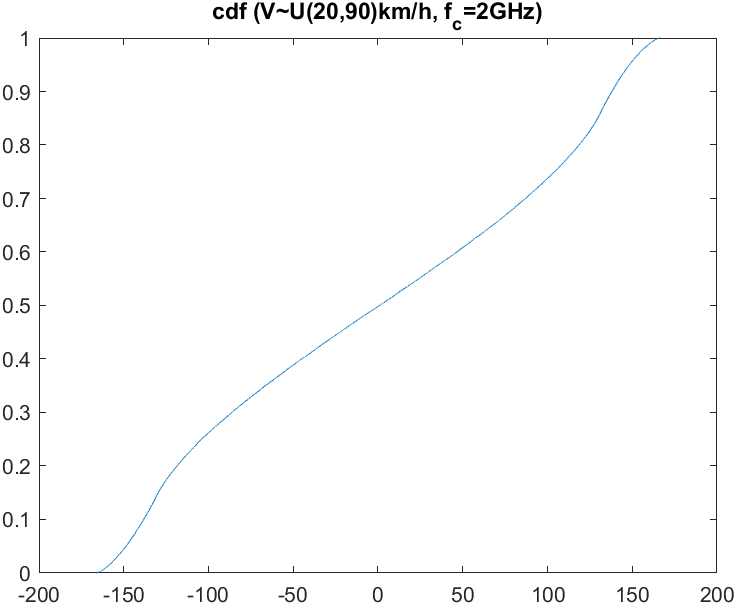
\includegraphics[width=0.49\textwidth]{(c)_cdf}}
\caption{$v\sim U(20,90)$km/h, $f_c$=2GHz}
\end{figure}


\item
Let $\Theta\sim U(-\pi,\pi),\  X\sim U(0,\pi)$,then, $\cos\Theta=\cos X$ since $\cos$ is even
Thus, consider $Y=f_m\cos X$\\
\begin{align}
F_Y(y)&=P(Y\leq y)\notag\\
&=P(f_m\cos X\leq y)\notag\\
&=P\left(X\geq \cos^{-1}\left(\frac{y}{f_m}\right)\right)\notag\\
&=P\left(X\leq \cos^{-1}\left(\frac{-y}{f_m}\right)\right)\notag\\
&=\frac{\cos^{-1}\left(\frac{-y}{f_m}\right)}{\pi}&{\rm for}\ y\in[-f_m,f_m] \notag\\
\Rightarrow f_Y(y)&=\frac{\partial}{\partial y}F_Y(y)\notag\\
&=\frac{1}{\pi f_m\sqrt{1-\left(\frac{y}{f_m}\right)^2}}\notag
\end{align}

\newpage

Now, take $v$=20km/h, $f_c$=2GHz to compare the corresponding $F_Y(y)$ and $ f_Y(y)$ with simulation of (a)
\begin{figure}[H]
\centering
\subfigure[pdf]{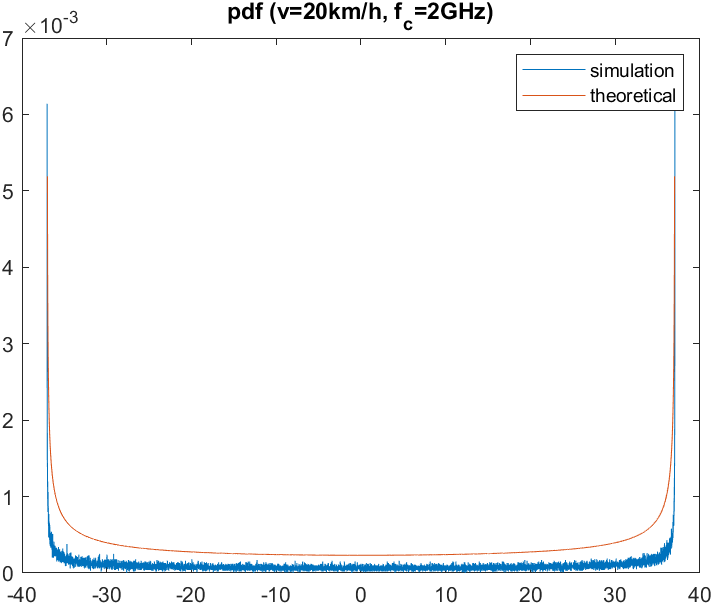
\includegraphics[width=0.49\textwidth]{(d)_pdf}}
\subfigure[cdf]{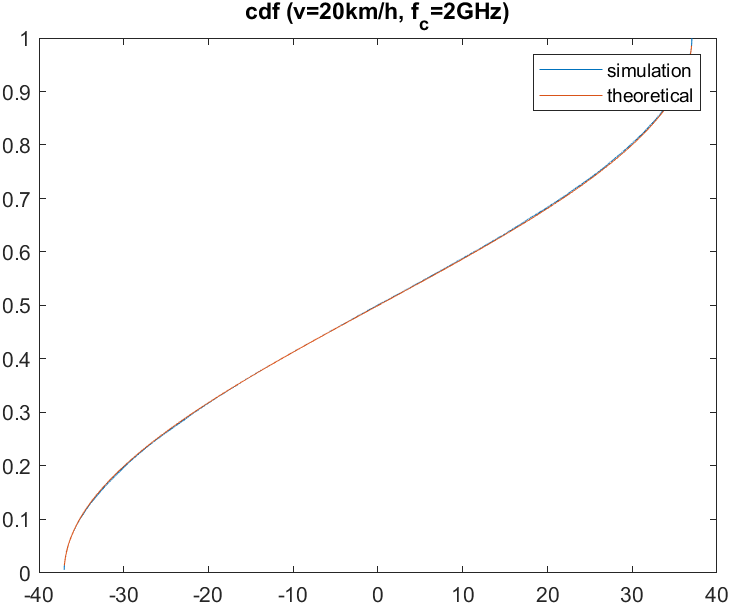
\includegraphics[width=0.49\textwidth]{(d)_cdf}}
\caption{compare theoretical result with simulation of (a)}
\end{figure}
Note that, since $f_Y(y)\rightarrow \infty $ as $y\rightarrow \pm 1$  in order to plot $f_Y(y)$ and the simulation pdf of (a) in one screen, I discard the points $(y,f_Y(y))$ that are near $\pm 1$ at first axis \\
Furthermore, the theoretical cdf and the simulative cdf are perfectly consistent but it is not the case for pdf. And it may be due to the fact that  $f_Y(y)\rightarrow \infty $ as $y\rightarrow \pm 1$ but simulation pdf can't approach  $ \infty$ no matter how near are $y$ and $\pm 1$ 



\end{enumerate}
\end{flushleft}

\end{document}